%%%%%%%%%%%%%%%%%%%%%%%%%%%%%%%%%%%%%%%%%%%%%%%%%%%%%%%%%
%%             东南大学数电实验报告 LaTeX 模板
%%                SEU-Circuit-Report.cls
%% https://github.com/Teddy-van-Jerry/SEU_Digital_Report
%% ======================================================
%% 版本信息:
%% v1.0 (Nov. 07, 2021)
%% ------------------------------------------------------
%% 模板制作:
%% Teddy van Jerry, (me@teddy-van-jerry.org)
%% * GitHub: https://github.com/Teddy-van-Jerry
%% * Website: https://teddy-van-jerry.org
%% * Blog: https://blog.teddy-van-jerry.org
%% ------------------------------------------------------
%% 使用说明:
%% 1. 编译使用 XeLaTeX 和 Biber
%% 2. 报告基本信息通过修改导言区以 exp 开头的命令
%% 3. 参考文献位于 ref/ref.bib
%% 4. 报告模板依据 MIT License 开源共享
%% ------------------------------------------------------
%% Copyright 2021 (c) Teddy van Jerry
%%
%% Permission is hereby granted, free of charge, to any
%% person obtaining a copy of this software and
%% associated documentation files (the "Software"), to
%% deal in the Software without restriction, including
%% without limitation the rights to use, copy, modify,
%% merge, publish, distribute, sublicense, and/or sell
%% copies of the Software, and to permit persons to whom
%% the Software is furnished to do so, subject to the
%% following conditions:
%%
%% The above copyright notice and this permission notice
%% shall be included in all copies or substantial
%% portions of the Software.
%% 
%% THE SOFTWARE IS PROVIDED "AS IS", WITHOUT WARRANTY OF
%% ANY KIND, EXPRESS OR IMPLIED, INCLUDING BUT NOT
%% LIMITED TO THE WARRANTIES OF MERCHANTABILITY, FITNESS
%% FOR A PARTICULAR PURPOSE AND NONINFRINGEMENT. IN NO
%% EVENT SHALL THE AUTHORS OR COPYRIGHT HOLDERS BE LIABLE
%% FOR ANY CLAIM, DAMAGES OR OTHER LIABILITY, WHETHER IN
%% AN ACTION OF CONTRACT, TORT OR OTHERWISE, ARISING
%% FROM, OUT OF OR IN CONNECTION WITH THE SOFTWARE OR THE
%% USE OR OTHER DEALINGS IN THE SOFTWARE.
%%%%%%%%%%%%%%%%%%%%%%%%%%%%%%%%%%%%%%%%%%%%%%%%%%%%%%%%%%

%% 使用实验报告模板类(字体大小 11pt 约为五号字)
\documentclass[11pt]{SEU-Digital-Report}

%%%%%%%%%%%%%%%%%%%% 报告基本信息 %%%%%%%%%%%%%%%%%%%%
\expno{三} % 实验序号
\expname{“简单”编程练习} % 实验名称
\expauthor{薛宇飞} % 姓名
\expID{04020235} % 学号
\expmates{} % 同组
\expmatesID{} % 学号(同组)
\expmajor{信息工程} % 专业
\explab{金智楼硬件实验室} % 实验室
\expdate{\today} % 实验日期
\expreportdate{\today} % 实验日期
\expgrade{} % 成绩评定
\exptutor{裴文江} % 评阅教师
%%%%%%%%%%%%%%%%%%%%%%%%%%%%%%%%%%%%%%%%%%%%%%%%%%%%
% \usepackage{xeCJK}
\usepackage{threeparttable} %table添加注释
\usepackage{colortbl}
\newcommand{\grayrow}{\rowcolor[rgb]{ .906, .902, .902}}
\usepackage{xcolor}  % tikz画图
\usepackage{tikz}  
\usetikzlibrary{arrows,shapes,chains} 
\usepackage{pgfplots}
\pgfplotsset{compat=1.11}

%% 报告正文
\begin{document}

% 打印封面页
\exptitlepage

\tableofcontents
\newpage

\section{实验目的与内容}       
\begin{enumerate}
    \item 结合实验教材\cite{book,guide},利用已掌握的宏汇编语言,进行简单的程序设计练习;
    \item 学习和掌握建立与运行汇编语言源程序各个步骤的命令;
    \item 熟悉汇编程序的调试过程。
\end{enumerate}

\section{实验预习任务}
在一个有正、负数的数据块中,找出负数的个数,假设有数据\texttt{-19,28,37,-46,55,61,-74},数据块的长度存放在\texttt{CX}寄存器中,负数的个数存放在以\texttt{SUM}为符号的单元中。
实验代码如下:
\begin{lstlisting}[language={[x86masm]Assembler},title=exp30.asm]
    DATA   SEGMENT
    NUM    DB -19,28,27,-46,55,61,-74
    SUM    DB ?
    DATA   ENDS

    MAIN SEGMENT
    ASSUME CS:MAIN,DS:DATA
    START: MOV  AX,DATA
           MOV  DS,AX
           MOV  CX,7
           MOV  AL,00
           LEA  SI,NUM  
    AGAIN: MOV  BL,[SI]
           CMP  BL,00
           JGE  NEXT
           INC  AL
    NEXT:  INC  SI
           LOOP AGAIN
           MOV  SUM,AL
           MOV  AH,4CH
           INT  21H
    MAIN ENDS
    END START    
\end{lstlisting}

实验流程如图 \ref{fig:usingmethod}:
\begin{figure}[hbpt]
    \centering
    \begin{tikzpicture}[node distance = 2cm]
    \definecolor{myblued}{RGB}{0,114,189}
    \definecolor{myred}{RGB}{217,83,25}
    \definecolor{myyellow}{RGB}{237,137,32}
    \definecolor{mypurple}{RGB}{126,47,142}
    \definecolor{myblues}{RGB}{77,190,238}
    \definecolor{mygreen}{RGB}{32,134,48}
      \pgfplotsset{
        label style = {font=\fontsize{9pt}{7.2}\selectfont},
        tick label style = {font=\fontsize{7pt}{7.2}\selectfont}
      }
    
    \small  % 字体大小
    \tikzstyle{format}=[rectangle,draw,thin,fill=white]  % 定义语句块的颜色,形状和边
    % rectangle:矩形,可加圆角(rounded corners,逗号跟在形状后面即可)
    % trapezium:平行四边形
    % diamond:菱形
    \tikzstyle{test}=[diamond,aspect=2,draw,thin]  % 定义条件块的形状,颜色
    \tikzstyle{point}=[coordinate,on grid,]  % 像素点,用于连接转移线

    % 定义note
    \node[format](asm){在记事本事先编好程序,并修改后缀名为\texttt{.asm}};
    \node[format,below of=asm,node distance=10mm](masm){使用命令\texttt{masm yourfile.asm}生成目标文件};
    \node[test,below of=masm,node distance=20mm](if){0 wornings, 0 errors?};
    \node[format,below of=if,node distance=20mm](link){使用命令\texttt{link yourfile}进行连接操作};
    \node[format,below of=link,node distance=10mm](execute){执行\texttt{youfile.exe}文件};
    % 开始画线
    \draw[->](asm)--(masm);
    \draw[->](masm)--(if);
    \draw[->](if)--node[left]{Yes}(link);
    \draw[->](link)--(execute);
    \draw[->](if.west) -+ (-5,-3) -+ node[left]{No}(-5,0) -- (asm.west);
    % \draw[-](point2) to [in=-90,out=90];
    % \draw[->](point2)--(asm.west);
\end{tikzpicture}
    
    \caption{执行流程}
    \label{fig:usingmethod}
\end{figure}

实验结果如图 \ref{fig:rlt0}所示:
\begin{figure}[htbp]
    \centering
    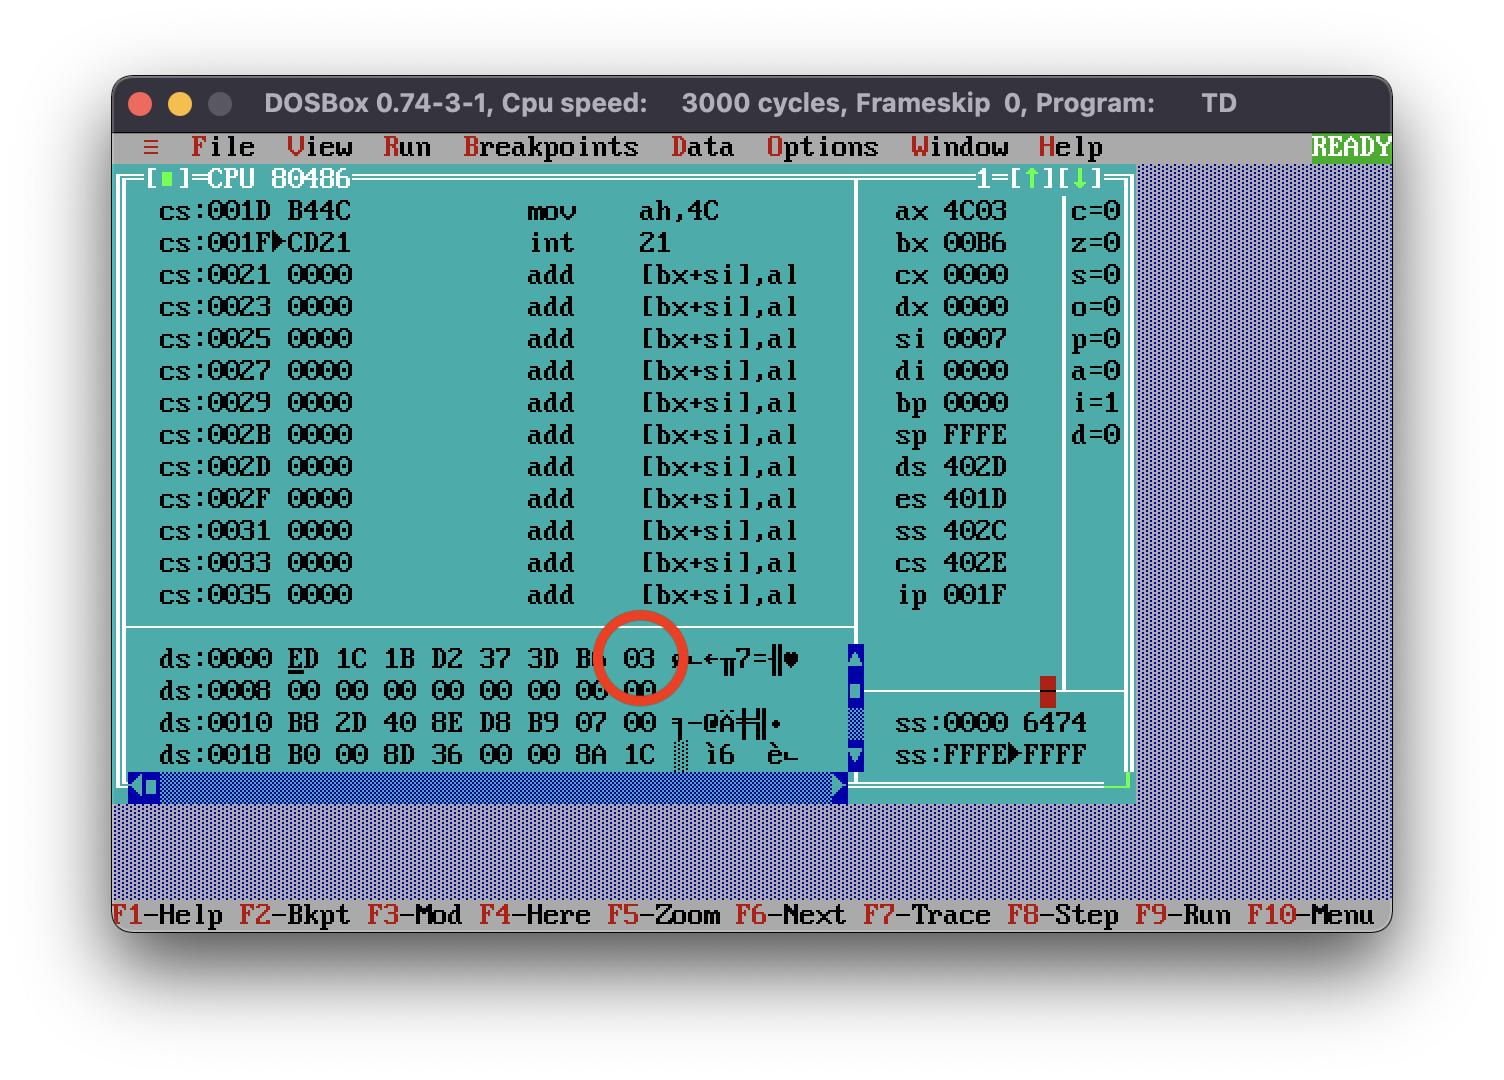
\includegraphics[width=0.7\textwidth]{fig/rlt0.png}
    \caption{预习实验结果}
    \label{fig:rlt0}
\end{figure}

\section{实验任务}
实验全部资料及完整代码详见薛宇飞的 \texttt{GitHub} 主页\cite{mygit}。具体实验任务如下:
\begin{enumerate}
    \item 在一个数据块中找出最大数:\\
    假设有数据22、46、32,72、84、16、156,且为不带符号的正 整数,数据块的长度存放在CX寄存器中,找出其中的最大数存放在以MAXN为符号的单元中。
    \item 求无符号字节数据之和,和数为8位二进制数:\\
    假设有数据38 、55、26、12、23,数据块的长度存放在CX寄存器中,和数存放在以SUM为符号的单元中。
    \item 求无符号字节数据之和,和数为16位二进制数:\\
    假设有数据58、25,45,73、64,43,数据块的长度存放在CX寄存器中,和数存放在以SUM为符号的字单元中。
    \item 求两个十进制数相乘的积$(53348\times 9)$,被乘数和乘数均以非压缩\texttt{BCD}码表示,并存放在内存中,乘积以非压缩\texttt{BCD}码的格式存放在以\texttt{SUM}为起始符号的单元中。
    \item 试分别用数据传送指令和串传送指令编写程序,将以\texttt{STR1}为首地址的字节存储单元中的数据\texttt{30H、31H、32H、33H、34H、35H、36H、37H、38H、39H、40H、41H、42H、43H、44H、45H},传送到以\texttt{STR2}为首地址的字节存储单元中。
    \item 假设任务1中的数据为有符号数,请找出其中的最大数存放在以\texttt{MAXN}为符号的单元中。
    \item 将任务4的乘积在屏幕上显示出来。
    \textcolor{red}{提示:}用DOS系统功能调用的字符串显示的功能。
\end{enumerate}
\textcolor{red}{要求:}上述所有任务的程序运行结束后,均要返回DOS。

\section{实验程序及分析}
\subsection{实验一}
实验流程如图 \ref{fig:exp31}:
\begin{figure}[hbpt]
    \centering
    \begin{tikzpicture}[node distance = 2cm]
    \definecolor{myblued}{RGB}{0,114,189}
    \definecolor{myred}{RGB}{217,83,25}
    \definecolor{myyellow}{RGB}{237,137,32}
    \definecolor{mypurple}{RGB}{126,47,142}
    \definecolor{myblues}{RGB}{77,190,238}
    \definecolor{mygreen}{RGB}{32,134,48}
      \pgfplotsset{
        label style = {font=\fontsize{9pt}{7.2}\selectfont},
        tick label style = {font=\fontsize{7pt}{7.2}\selectfont}
      }
    
    \small  % 字体大小
    \tikzstyle{format}=[rectangle,draw,thin,fill=white]  % 定义语句块的颜色,形状和边
    % rectangle:矩形,可加圆角(rounded corners,逗号跟在形状后面即可)
    % trapezium:平行四边形
    % diamond:菱形
    \tikzstyle{test}=[diamond,aspect=2,draw,thin]  % 定义条件块的形状,颜色
    \tikzstyle{point}=[coordinate,on grid,]  % 像素点,用于连接转移线

    % 定义note
    \node[format](init){初始化数据段,将数据传入\texttt{DS}};
    \node[format,below of=init,node distance=10mm](1){定义数据指针\texttt{BX},设置循环次数};
    \node[format,below of=1,node distance=10mm](2){假设第一个数据是最大值,放入\texttt{AL}};
    \node[format,below of=2,node distance=10mm](3){\texttt{BX+1}};
    \node[format,below of=3,node distance=10mm](4){使用\texttt{CPM}指令比较数据,表现在标志位};
    \node[test,below of=4,node distance=20mm](5){\texttt{AL<[BX]?(无符号数比较)}};
    \node[format,below of=5,node distance=20mm](6){更新\texttt{AL}为\texttt{[BX]}};
    \node[test,below of=6,node distance=20mm](7){是否完成预设循环次数?};
    \node[format,below of=7,node distance=20mm](8){保存结果};
    \node[format,below of=8,node distance=10mm](end){结束,返回\texttt{DOS}};
    % 开始画线
    \draw[->](init)--(1);
    \draw[->](1)--(2);
    \draw[->](2)--(3);
    \draw[->](3)--(4);
    \draw[->](4)--(5);
    \draw[->](5)--node[left]{Yes}(6);
    \draw[->](6)--(7);
    \draw[->](7)--node[left]{Yes}(8);
    \draw[->](8)--(end);
    \draw[->](5.west) -+ (-4,-6) -+ node[left]{No}(-4,-10) -- (7.west);
    \draw[->](7.east) -+ (+4,-10) -+ node[right]{No}(+4,-3) -- (3.east);
\end{tikzpicture}

    \caption{执行流程}
    \label{fig:exp31}
\end{figure}


实验要求代码、正确结果(图\ref{fig:rlt1})如下:
\begin{lstlisting}[language={[x86masm]Assembler},title=exp31.asm]
    DATA   SEGMENT
    NUM    DB 22,46,32,72,84,16,156  ;定义数据段
    MAXN   DB ?  ;定义结果存放处
    DATA   ENDS

    MAIN SEGMENT 
    ASSUME CS:MAIN,DS:DATA
    START: MOV  AX,DATA
           MOV  DS,AX     ;DATA数据段传入DS
           LEA  BX,NUM    ;获取NUM偏移地址,传入指针BX
           MOV  CX,06     ;循环次数为6
           MOV  AL ,[BX]  ;初始假设第一个数据是最大值
    AGAIN: INC  BX        ;BX指针后移1位
           CMP  AL,[BX]   ;比较数据大小并更新标志位
           JNBE NEXT      ;如果AL>[BX],跳转至NEXT
           MOV  AL,[BX]   ;如果AL<[BX],更新AL
    NEXT:  LOOP AGAIN     ;循环CX次
           MOV  MAXN,AL   ;将结果存入MAXN
           MOV  AH,4CH
           INT  21H
    MAIN ENDS
    END START
\end{lstlisting}

\begin{figure}[htbp]
    \centering
    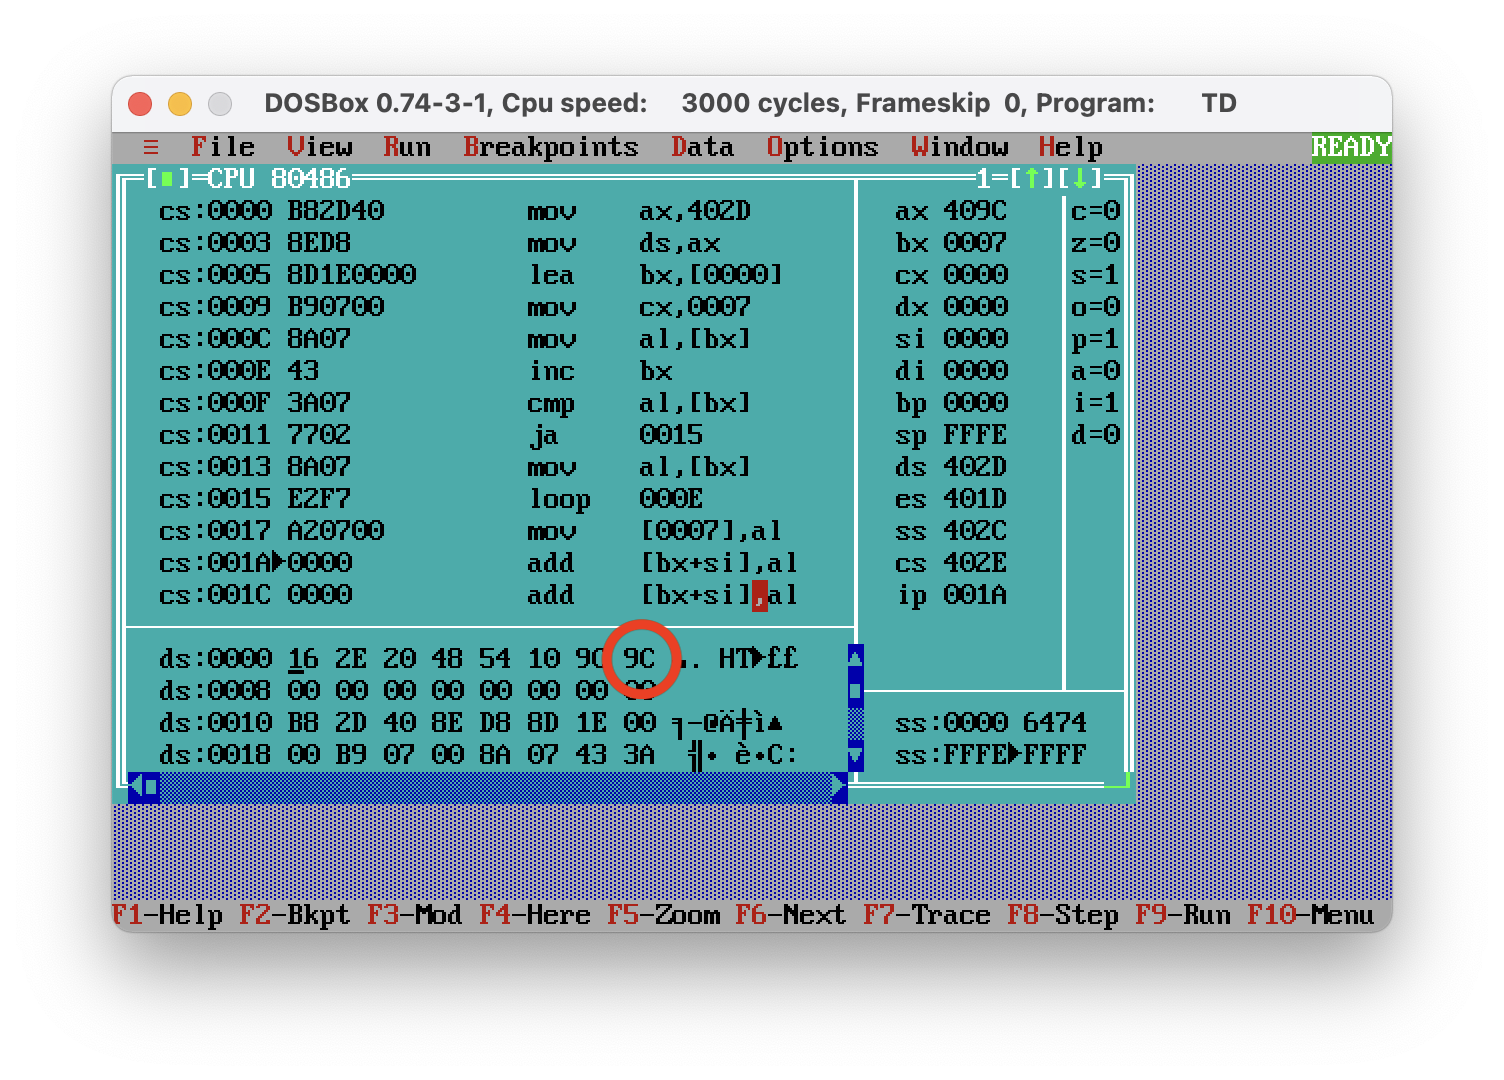
\includegraphics[width=0.7\textwidth]{fig/rlt1.png}
    \caption{实验结果}
    \label{fig:rlt1}
\end{figure}

\begin{note}{\texttt{JA/JNBE}用法小结}{}
    与\texttt{CPM}指令配合使用,严格大于时候跳转。
\end{note}

\subsection{实验二}
实验流程如图 \ref{fig:exp32}:
\begin{figure}[hbpt]
    \centering
    \begin{tikzpicture}[node distance = 2cm]
    \definecolor{myblued}{RGB}{0,114,189}
    \definecolor{myred}{RGB}{217,83,25}
    \definecolor{myyellow}{RGB}{237,137,32}
    \definecolor{mypurple}{RGB}{126,47,142}
    \definecolor{myblues}{RGB}{77,190,238}
    \definecolor{mygreen}{RGB}{32,134,48}
      \pgfplotsset{
        label style = {font=\fontsize{9pt}{7.2}\selectfont},
        tick label style = {font=\fontsize{7pt}{7.2}\selectfont}
      }
    
    \small  % 字体大小
    \tikzstyle{format}=[rectangle,draw,thin,fill=white]  % 定义语句块的颜色,形状和边
    % rectangle:矩形,可加圆角(rounded corners,逗号跟在形状后面即可)
    % trapezium:平行四边形
    % diamond:菱形
    \tikzstyle{test}=[diamond,aspect=2,draw,thin]  % 定义条件块的形状,颜色
    \tikzstyle{point}=[coordinate,on grid,]  % 像素点,用于连接转移线

    % 定义note
    \node[format](init){初始化数据段,将数据传入\texttt{DS}};
    \node[format,below of=init,node distance=10mm](1){定义数据指针\texttt{BX},设置循环次数};
    \node[format,below of=1,node distance=10mm](2){对存放结果的\texttt{AL}清零};
    \node[format,below of=2,node distance=10mm](3){将新数据加在结果存放处};
    \node[format,below of=3,node distance=10mm](4){指针+1};
    \node[test,below of=4,node distance=20mm](5){是否达到循环次数?};
    \node[format,below of=5,node distance=20mm](6){保存结果};
    \node[format,below of=6,node distance=10mm](end){结束,返回\texttt{DOS}};
    % 开始画线
    \draw[->](init)--(1);
    \draw[->](1)--(2);
    \draw[->](2)--(3);
    \draw[->](3)--(4);
    \draw[->](4)--(5);
    \draw[->](5)--node[left]{Yes}(6);
    \draw[->](6)--(end);
    \draw[->](5.west) -+ (-4,-6) -+ node[left]{No}(-4,-3) -- (3.west);
\end{tikzpicture}

    \caption{执行流程}
    \label{fig:exp32}
\end{figure}

实验要求代码、正确结果(图\ref{fig:rlt2})如下:
\begin{lstlisting}[language={[x86masm]Assembler},title=exp32.asm]
    DATA   SEGMENT
    NUM    DB 38,55,26,12,23  
    SUM    DB ?
    DATA   ENDS

    CODE SEGMENT
    ASSUME CS:CODE,DS:DATA
    START: MOV  AX,DATA   
           MOV  DS,AX    ;DATA数据段传入DS
           MOV  CX,05    ;设置循环次数
           LEA  BX,NUM   ;取NUM的地址给BX
           SUB  AL,AL    ;将存放结果的AL清零
    NEXT:  ADD  AL,[BX]  ;添加数据
           INC  BX       ;指针加1
           LOOP NEXT     ;循环,次数为CX
           MOV  SUM,AL   ;储存结果
           MOV  AH,4CH
           INT  21H
    CODE ENDS
    END START
\end{lstlisting}

\begin{figure}[htbp]
    \centering
    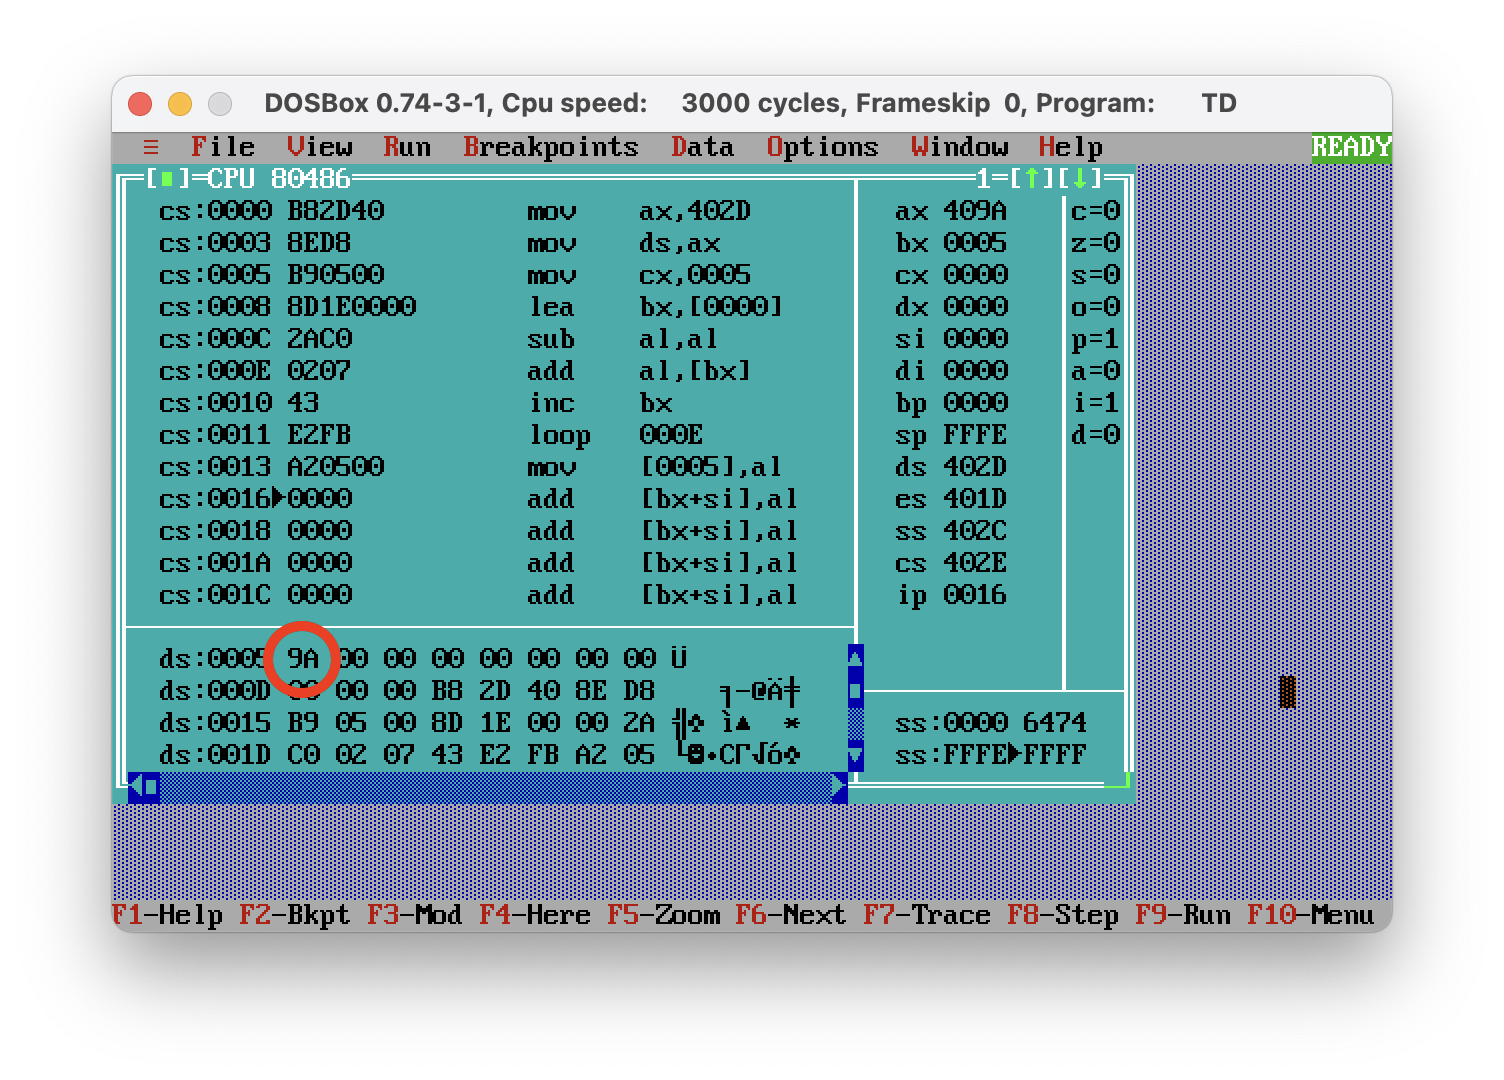
\includegraphics[width=0.7\textwidth]{fig/rlt2.png}
    \caption{实验结果}
    \label{fig:rlt2}
\end{figure}

\subsection{实验三}
实验流程如图 \ref{fig:exp33}:
\begin{figure}[hbpt]
    \centering
    \begin{tikzpicture}[node distance = 2cm]
    \definecolor{myblued}{RGB}{0,114,189}
    \definecolor{myred}{RGB}{217,83,25}
    \definecolor{myyellow}{RGB}{237,137,32}
    \definecolor{mypurple}{RGB}{126,47,142}
    \definecolor{myblues}{RGB}{77,190,238}
    \definecolor{mygreen}{RGB}{32,134,48}
      \pgfplotsset{
        label style = {font=\fontsize{9pt}{7.2}\selectfont},
        tick label style = {font=\fontsize{7pt}{7.2}\selectfont}
      }
    
    \small  % 字体大小
    \tikzstyle{format}=[rectangle,draw,thin,fill=white]  % 定义语句块的颜色,形状和边
    % rectangle:矩形,可加圆角(rounded corners,逗号跟在形状后面即可)
    % trapezium:平行四边形
    % diamond:菱形
    \tikzstyle{test}=[diamond,aspect=2,draw,thin]  % 定义条件块的形状,颜色
    \tikzstyle{point}=[coordinate,on grid,]  % 像素点,用于连接转移线

    % 定义note
    \node[format](init){初始化数据段,将数据传入\texttt{DS}};
    \node[format,below of=init,node distance=10mm](1){设置循环次数};
    \node[format,below of=1,node distance=10mm](2){对存放结果的\texttt{AX}清零};
    \node[format,below of=2,node distance=10mm](3){将新数据加在\texttt{AL}完成低位加法};
    \node[format,below of=3,node distance=10mm](4){调整上一次加法可能产生的进位};
    \node[format,below of=4,node distance=10mm](5){数据指针\texttt{+1}};
    \node[test,below of=5,node distance=20mm](6){是否达到循环次数?};
    \node[format,below of=6,node distance=20mm](7){保存结果};
    \node[format,below of=7,node distance=10mm](end){结束,返回\texttt{DOS}};
    % 开始画线
    \draw[->](init)--(1);
    \draw[->](1)--(2);
    \draw[->](2)--(3);
    \draw[->](3)--(4);
    \draw[->](4)--(5);
    \draw[->](5)--(6);
    \draw[->](6)--node[left]{Yes}(7);
    \draw[->](7)--(end);
    \draw[->](6.west) -+ (-4,-7) -+ node[left]{No}(-4,-3) -- (3.west);
\end{tikzpicture}

    \caption{执行流程}
    \label{fig:exp33}
\end{figure}

实验要求代码、正确结果(图\ref{fig:rlt3})如下:
\begin{lstlisting}[language={[x86masm]Assembler},title=exp33.asm]
    DATA   SEGMENT
    NUM    DB 58,25,45,73,64,43
    SUM    DW ?    
    DATA   ENDS

    CODE SEGMENT
    ASSUME CS:CODE,DS:DATA
    START: MOV  AX,DATA   
           MOV  DS,AX    ;将DATA数据传入DS
           LEA  BX,NUM   ;NUM地址传送给BX
           MOV  CX,6     ;循环次数为6
           SUB  AX,AX    ;AX清零
    NEXT:  ADD  AL,[BX]  ;这里用于低位的加法   
           ADC  AH,0     ;上一步加法可能会进位在这一步加进来
           INC  BX       ;指针加1
           LOOP NEXT     ;循环CX次
           MOV  SUM,AX   ;传送结果
           MOV  AH,4CH
           INT  21H
    CODE ENDS
    END START
\end{lstlisting}

\begin{figure}[htbp]
    \centering
    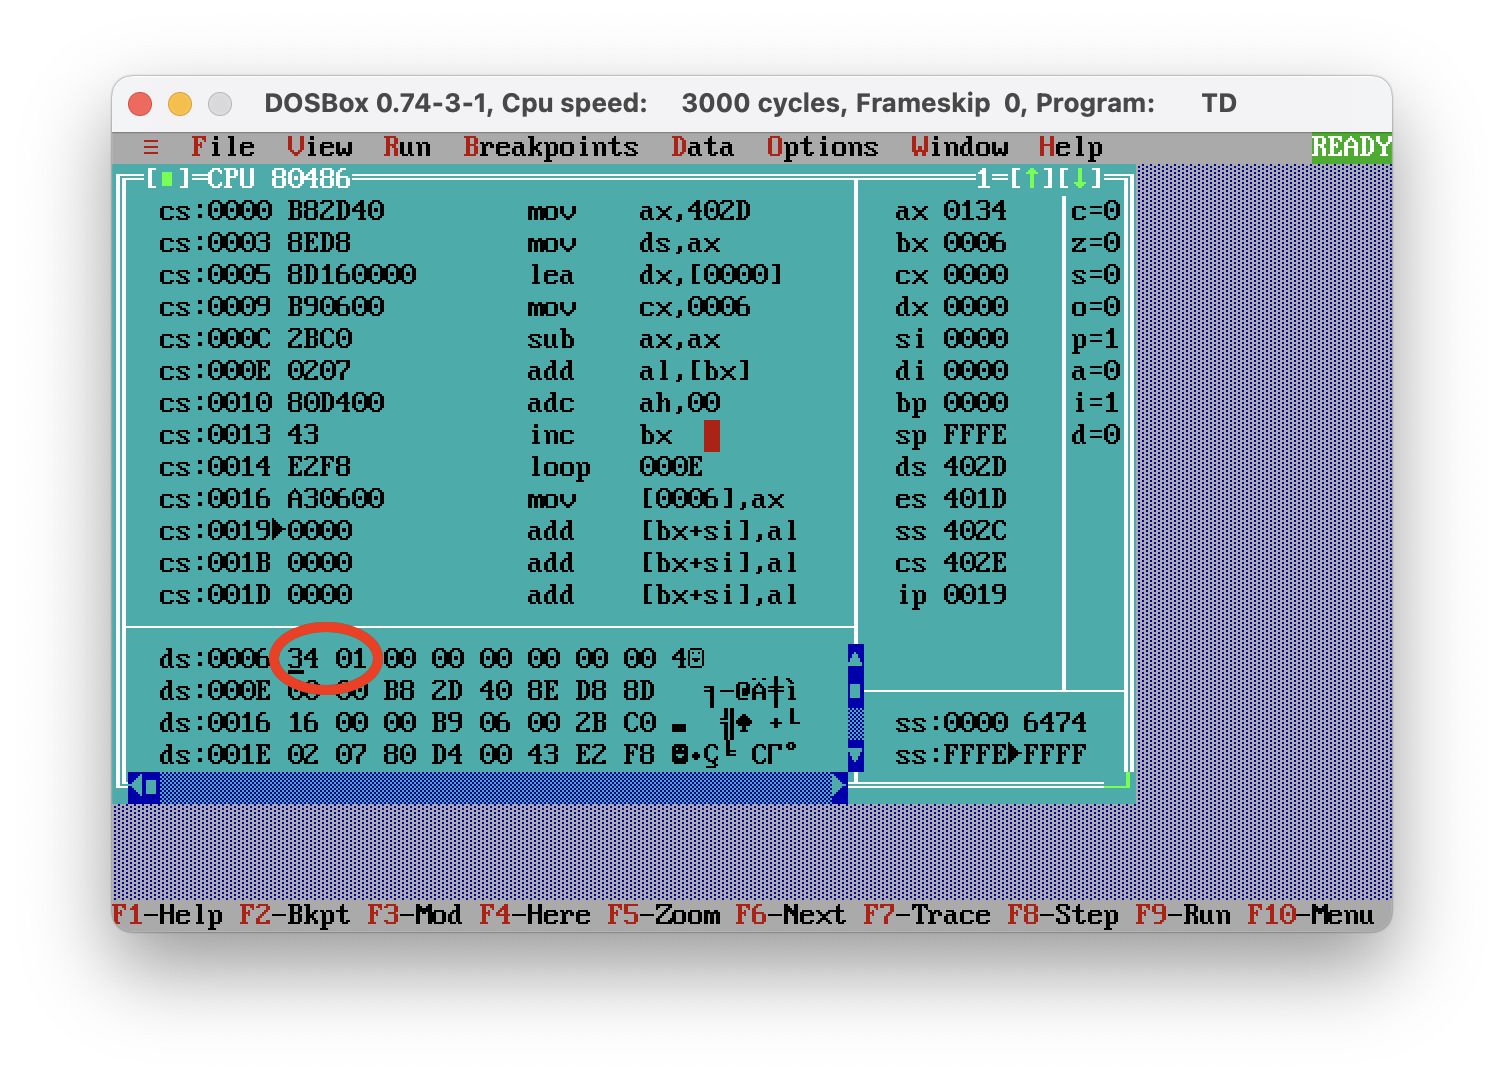
\includegraphics[width=0.7\textwidth]{fig/rlt3.png}
    \caption{实验结果}
    \label{fig:rlt3}
\end{figure}

\begin{note}{\texttt{ADC}指令}{}
    \texttt{ADC AH,0}通过加0并加符号为来将符号位考虑进去。
\end{note}

\subsection{实验四}
实验流程如图 \ref{fig:exp34}:
\begin{figure}[hbpt]
    \centering
    \begin{tikzpicture}[node distance = 2cm]
    \definecolor{myblued}{RGB}{0,114,189}
    \definecolor{myred}{RGB}{217,83,25}
    \definecolor{myyellow}{RGB}{237,137,32}
    \definecolor{mypurple}{RGB}{126,47,142}
    \definecolor{myblues}{RGB}{77,190,238}
    \definecolor{mygreen}{RGB}{32,134,48}
      \pgfplotsset{
        label style = {font=\fontsize{9pt}{7.2}\selectfont},
        tick label style = {font=\fontsize{7pt}{7.2}\selectfont}
      }
    
    \small  % 字体大小
    \tikzstyle{format}=[rectangle,draw,thin,fill=white]  % 定义语句块的颜色,形状和边
    % rectangle:矩形,可加圆角(rounded corners,逗号跟在形状后面即可)
    % trapezium:平行四边形
    % diamond:菱形
    \tikzstyle{test}=[diamond,aspect=2,draw,thin]  % 定义条件块的形状,颜色
    \tikzstyle{point}=[coordinate,on grid,]  % 像素点,用于连接转移线

    % 定义note
    \node[format](init){初始化数据段,将数据传入\texttt{DS}};
    \node[format,below of=init,node distance=10mm](1){设置结果数组位置\texttt{[DI]}、被乘数数组的位置、循环次数};
    \node[format,below of=1,node distance=10mm](2){把此时指针所指的数字搬到\texttt{AL}};
    \node[format,below of=2,node distance=10mm](3){被乘数指针\texttt{+1}};
    \node[format,below of=3,node distance=10mm](4){进行相乘操作};
    \node[format,below of=4,node distance=10mm](5){非压缩\texttt{BCD}码的调整乘法};
    \node[format,below of=5,node distance=10mm](6){将[DI]中算出来的上一位的进位加上};
    \node[format,below of=6,node distance=10mm](7){非压缩\texttt{BCD}码的调整加法};
    \node[format,below of=7,node distance=10mm](8){调整好的正确的低位给了\texttt{[DI]}};
    \node[format,below of=8,node distance=10mm](9){结果指针\texttt{+1}};
    \node[format,below of=9,node distance=10mm](10){把调整好的正确的进位给了\texttt{[DI]}};
    \node[test,below of=10,node distance=20mm](11){是否达到循环次数?};
    \node[format,below of=11,node distance=20mm](end){结束,返回\texttt{DOS}};
    % 开始画线
    \draw[->](init)--(1);
    \draw[->](1)--(2);
    \draw[->](2)--(3);
    \draw[->](3)--(4);
    \draw[->](4)--(5);
    \draw[->](5)--(6);
    \draw[->](6)--(7);
    \draw[->](7)--(8);
    \draw[->](8)--(9);
    \draw[->](9)--(10);
    \draw[->](10)--(11);
    \draw[->](11)--node[left]{Yes}(end);
    \draw[->](11.west) -+ (-4,-12) -+ node[left]{No}(-4,-2) -- (2.west);
\end{tikzpicture}

    \caption{执行流程}
    \label{fig:exp34}
\end{figure}

实验要求代码、正确结果(图\ref{fig:rlt4})如下:
\begin{lstlisting}[language={[x86masm]Assembler},title=exp34.asm]
    DATA   SEGMENT
    DATA1  DB 08,04,03,03,05
    DATA2  DB 09
    SUM    DB 6 DUP(00)   ;把00复制6次,占用6个BYTE
    DATA   ENDS 
      
    CODE SEGMENT
    ASSUME CS:CODE,DS:DATA
    START: MOV AX,DATA          
           MOV DS,AX             ;手动分配段地址
           MOV SI,OFFSET DATA2   ;DATA2的偏移地址给了SI
           MOV DL,[SI]           ;把SI内所指向的存储器的内容给了DL
           MOV SI,OFFSET DATA1   ;DATA1的偏移地址给了SI
           MOV DI,OFFSET SUM     ;SUM的偏移地址给了DI
           MOV CX,05             ;循环次数为5
    NEXT:  MOV AL,[SI]           ;一位位开始算,先从第一位开始
           INC SI                ;指针加一,指向下一位
           MUL DL                ;和09相乘
           AAM                   ;非压缩BCD码的乘法调整指令
           ADD AL,[DI]           ;[DI]中有上一个算出来的进位,先把进位加上
           AAA                   ;调整成非压缩BCD码
           MOV [DI],AL           ;调整好之后,把正确的低位给了[DI]
           INC DI                ;存放下一个数字的位置
           MOV [DI],AH           ;把上一个调整产生的进位放到DI中
           LOOP NEXT
           MOV  AH,4CH
           INT  21H
    CODE ENDS
    END START     
\end{lstlisting}

\begin{figure}[htbp]
    \centering
    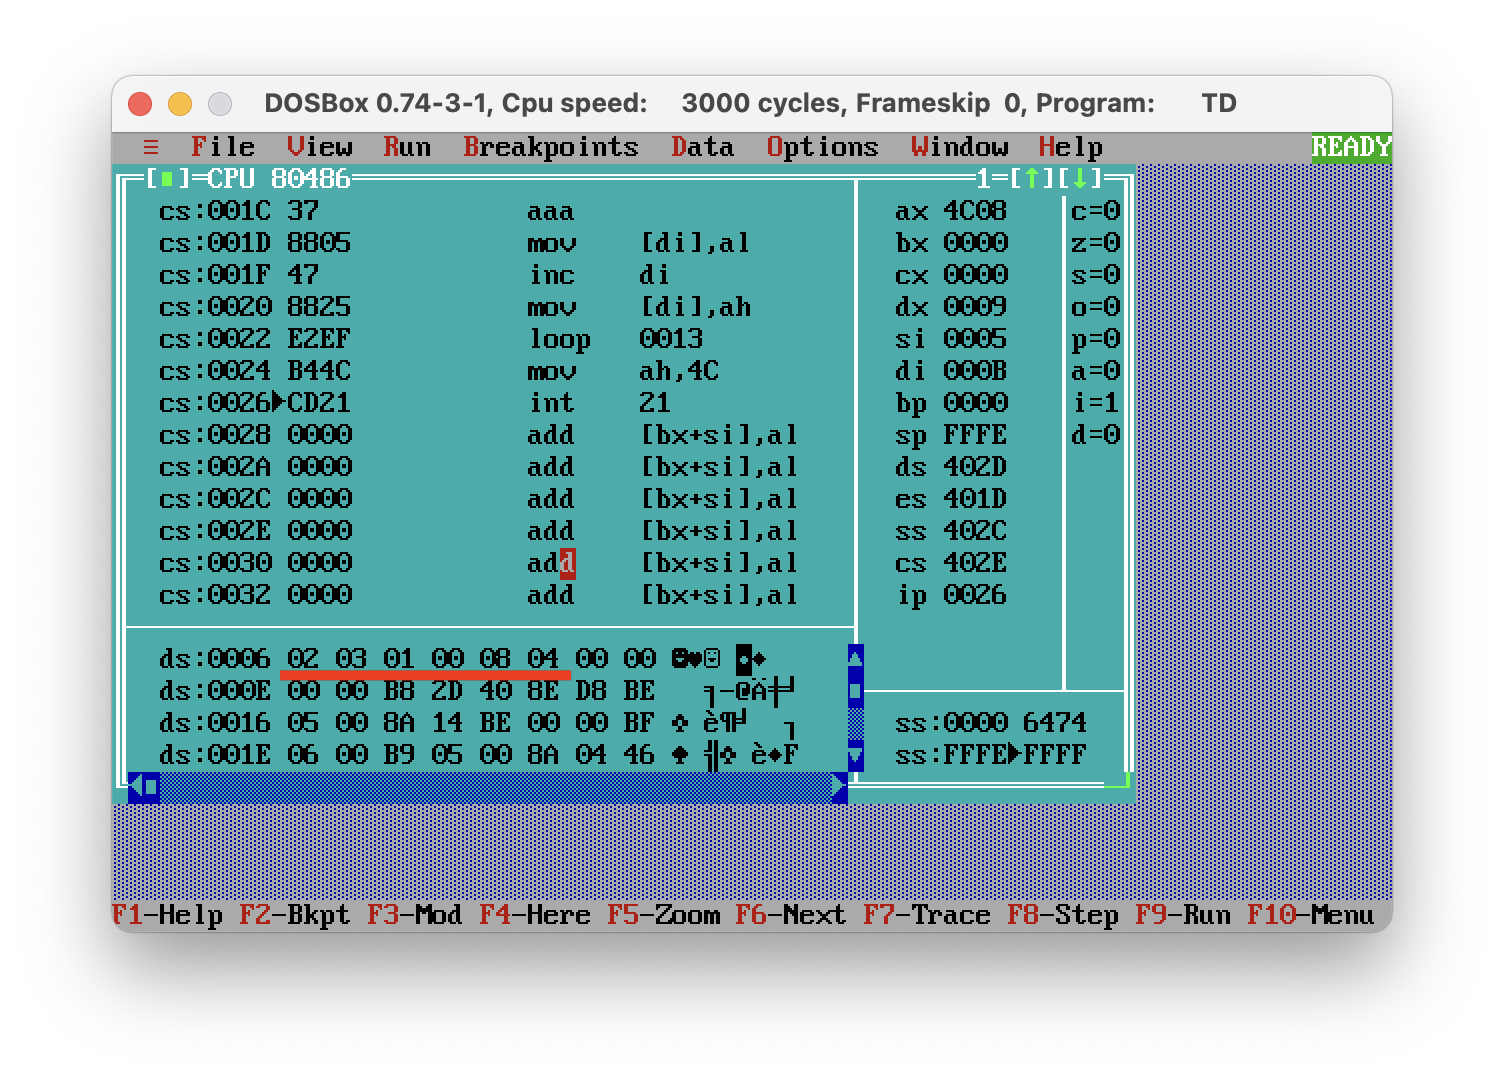
\includegraphics[width=0.7\textwidth]{fig/rlt4.png}
    \caption{实验结果}
    \label{fig:rlt4}
\end{figure}

\subsection{实验五}
子实验1流程如图 \ref{fig:exp351}:
\begin{figure}[hbpt]
    \centering
    \begin{tikzpicture}[node distance = 2cm]
    \definecolor{myblued}{RGB}{0,114,189}
    \definecolor{myred}{RGB}{217,83,25}
    \definecolor{myyellow}{RGB}{237,137,32}
    \definecolor{mypurple}{RGB}{126,47,142}
    \definecolor{myblues}{RGB}{77,190,238}
    \definecolor{mygreen}{RGB}{32,134,48}
      \pgfplotsset{
        label style = {font=\fontsize{9pt}{7.2}\selectfont},
        tick label style = {font=\fontsize{7pt}{7.2}\selectfont}
      }
    
    \small  % 字体大小
    \tikzstyle{format}=[rectangle,draw,thin,fill=white]  % 定义语句块的颜色,形状和边
    % rectangle:矩形,可加圆角(rounded corners,逗号跟在形状后面即可)
    % trapezium:平行四边形
    % diamond:菱形
    \tikzstyle{test}=[diamond,aspect=2,draw,thin]  % 定义条件块的形状,颜色
    \tikzstyle{point}=[coordinate,on grid,]  % 像素点,用于连接转移线

    % 定义note
    \node[format](init){初始化数据段,将数据传入\texttt{DS}};
    \node[format,below of=init,node distance=10mm](1){设置循环次数、源数组位置、目标数组位置};
    \node[format,below of=1,node distance=10mm](2){把对应源数据放到对应目标数据位置上};%
    \node[format,below of=2,node distance=10mm](3){源数组、目标数组指针都加1};
    \node[test,below of=3,node distance=20mm](4){是否达到循环次数?};%
    \node[format,below of=4,node distance=20mm](end){结束,返回\texttt{DOS}};
    % 开始画线
    \draw[->](init)--(1);
    \draw[->](1)--(2);
    \draw[->](2)--(3);
    \draw[->](3)--(4);
    \draw[->](4)--node[left]{Yes}(end);
    \draw[->](4.west) -+ (-4,-5) -+ node[left]{No}(-4,-2) -- (2.west);
\end{tikzpicture}

    \caption{执行流程}
    \label{fig:exp351}
\end{figure}
子实验2流程如图 \ref{fig:exp352}:
\begin{figure}[hbpt]
    \centering
    \begin{tikzpicture}[node distance = 2cm]
    \definecolor{myblued}{RGB}{0,114,189}
    \definecolor{myred}{RGB}{217,83,25}
    \definecolor{myyellow}{RGB}{237,137,32}
    \definecolor{mypurple}{RGB}{126,47,142}
    \definecolor{myblues}{RGB}{77,190,238}
    \definecolor{mygreen}{RGB}{32,134,48}
      \pgfplotsset{
        label style = {font=\fontsize{9pt}{7.2}\selectfont},
        tick label style = {font=\fontsize{7pt}{7.2}\selectfont}
      }
    
    \small  % 字体大小
    \tikzstyle{format}=[rectangle,draw,thin,fill=white]  % 定义语句块的颜色,形状和边
    % rectangle:矩形,可加圆角(rounded corners,逗号跟在形状后面即可)
    % trapezium:平行四边形
    % diamond:菱形
    \tikzstyle{test}=[diamond,aspect=2,draw,thin]  % 定义条件块的形状,颜色
    \tikzstyle{point}=[coordinate,on grid,]  % 像素点,用于连接转移线

    % 定义note
    \node[format](init){初始化数据段,将数据传入\texttt{DS、ES}};
    \node[format,below of=init,node distance=10mm](1){设置循环次数、源串地址、目标串地址};
    \node[format,below of=1,node distance=10mm](2){把对应源数据放到对应目标数据位置上};
    \node[format,below of=2,node distance=10mm](3){使用\texttt{CLD}命令将\texttt{DF}清零,让指针递增};
    \node[format,below of=3,node distance=10mm](4){使用串操作指令,自动完成复制};
    \node[format,below of=4,node distance=10mm](end){结束,返回\texttt{DOS}};
    % 开始画线
    \draw[->](init)--(1);
    \draw[->](1)--(2);
    \draw[->](2)--(3);
    \draw[->](3)--(4);
    \draw[->](4)--(end);
\end{tikzpicture}

    \caption{执行流程}
    \label{fig:exp352}
\end{figure}

实验要求代码、正确结果(图\ref{fig:rlt5}以及图\ref{fig:rlt55})如下:
\begin{lstlisting}[language={[x86masm]Assembler},title=exp351.asm]
    DATA  SEGMENT
    STR1  DB 30H,31H,32H,33H,34H
          DB 35H,36H,37H,38H,39H
          DB 40H,41H,42H,43H,44H,45H
    COUNT EQU $-STR1        ;定义数据长度
    STR2  DB COUNT DUP(0)   ;复制产生一个一样长度的数据段
    DATA  ENDS
    
    CODE SEGMENT
    ASSUME DS:DATA,CS:CODE
    START: MOV AX,DATA
           MOV DS,AX
           LEA SI,STR1   ;源数组
           LEA DI,STR2   ;目标数组
           MOV CX,COUNT  ;数据个数复制给CX
    NEXT:  MOV AL,[SI]
           MOV [DI],AL   ;通过AL寄存器间接传递
           INC SI        
           INC DI        ;指针加1
           LOOP NEXT
           MOV AH,4CH
           INT 21H
    CODE ENDS
    END START    
\end{lstlisting}

\begin{lstlisting}[language={[x86masm]Assembler},title=exp352.asm]
    DATA  SEGMENT
    STR1  DB 30H,31H,32H,33H,34H,35H,36H,37H
          DB 38H,39H,40H,41H,42H,43H,44H,45H
    COUNT EQU $-STR1
    STR2  DB COUNT DUP(?)    
    DATA  ENDS
    
    CODE SEGMENT    
    ASSUME DS:DATA,ES:DATA,CS:CODE
    START: MOV AX,DATA
           MOV DS,AX    
           MOV ES,AX    ;初始化DS和ES
           LEA SI,STR1
           LEA DI,STR2  ;初始化源串和目标串地址
           MOV CX,COUNT ;初始化串长度
           CLD          ;DF清零表示指针+
           REP MOVSB    ;重复移动
           MOV AH,4CH
           INT 21H
    CODE ENDS
    END START    
\end{lstlisting}

\begin{figure}[htbp]
    \centering
    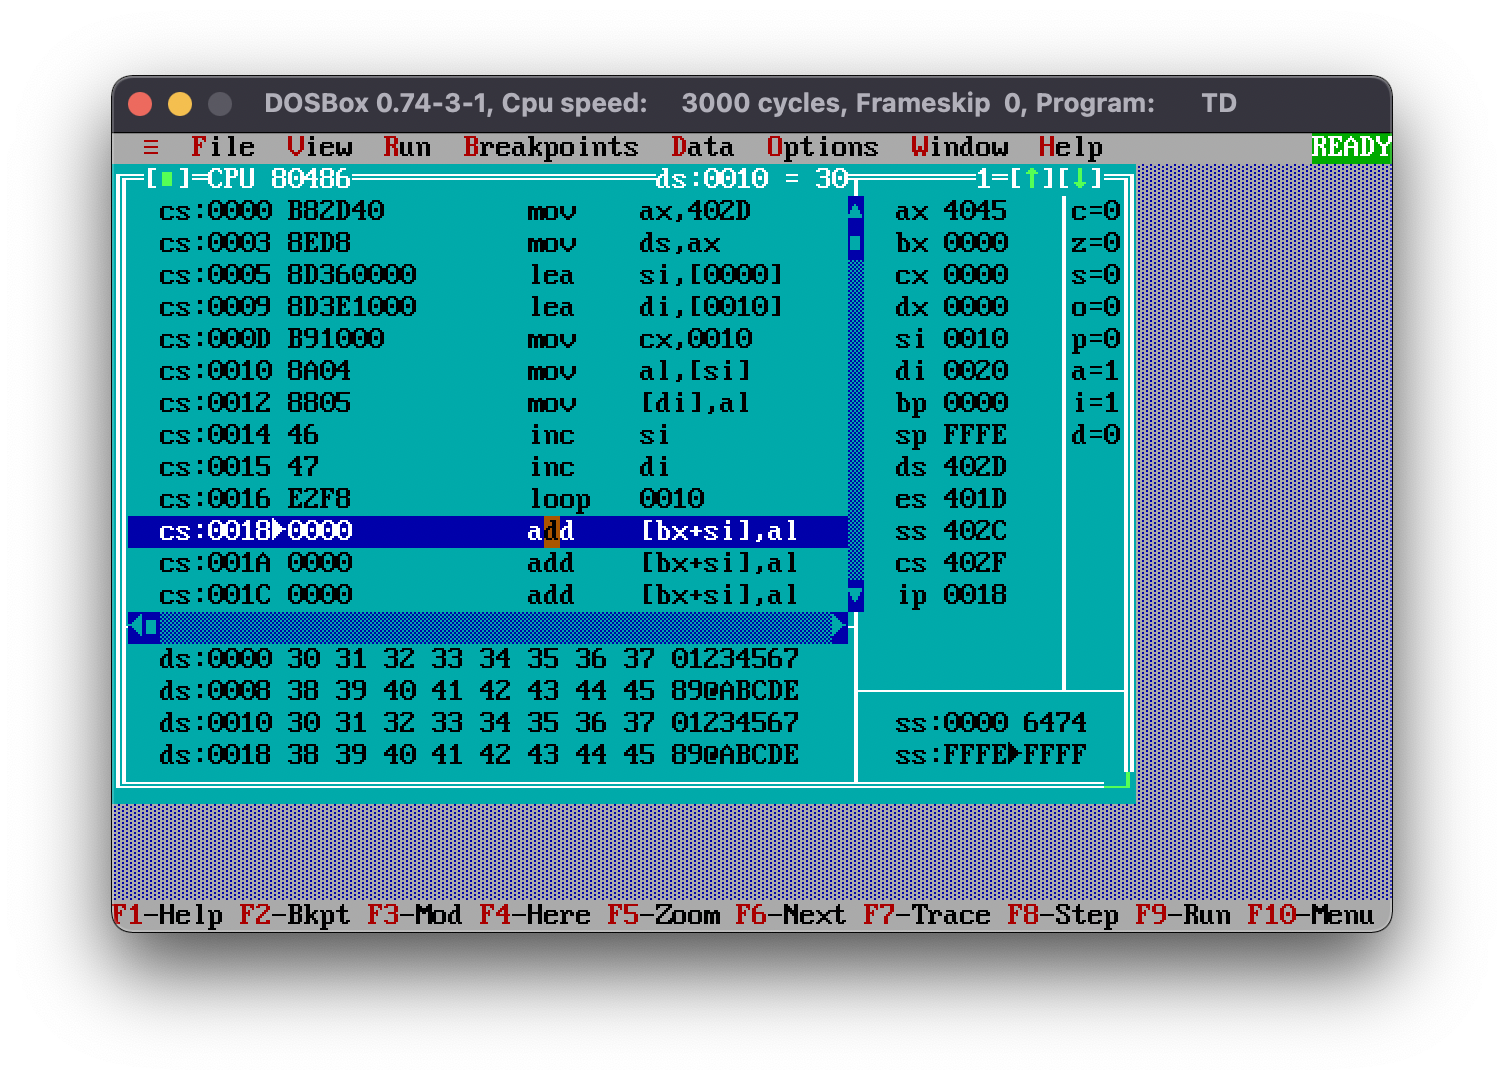
\includegraphics[width=0.7\textwidth]{fig/rlt5.png}
    \caption{实验结果}
    \label{fig:rlt5}
\end{figure}

\begin{figure}[htbp]
    \centering
    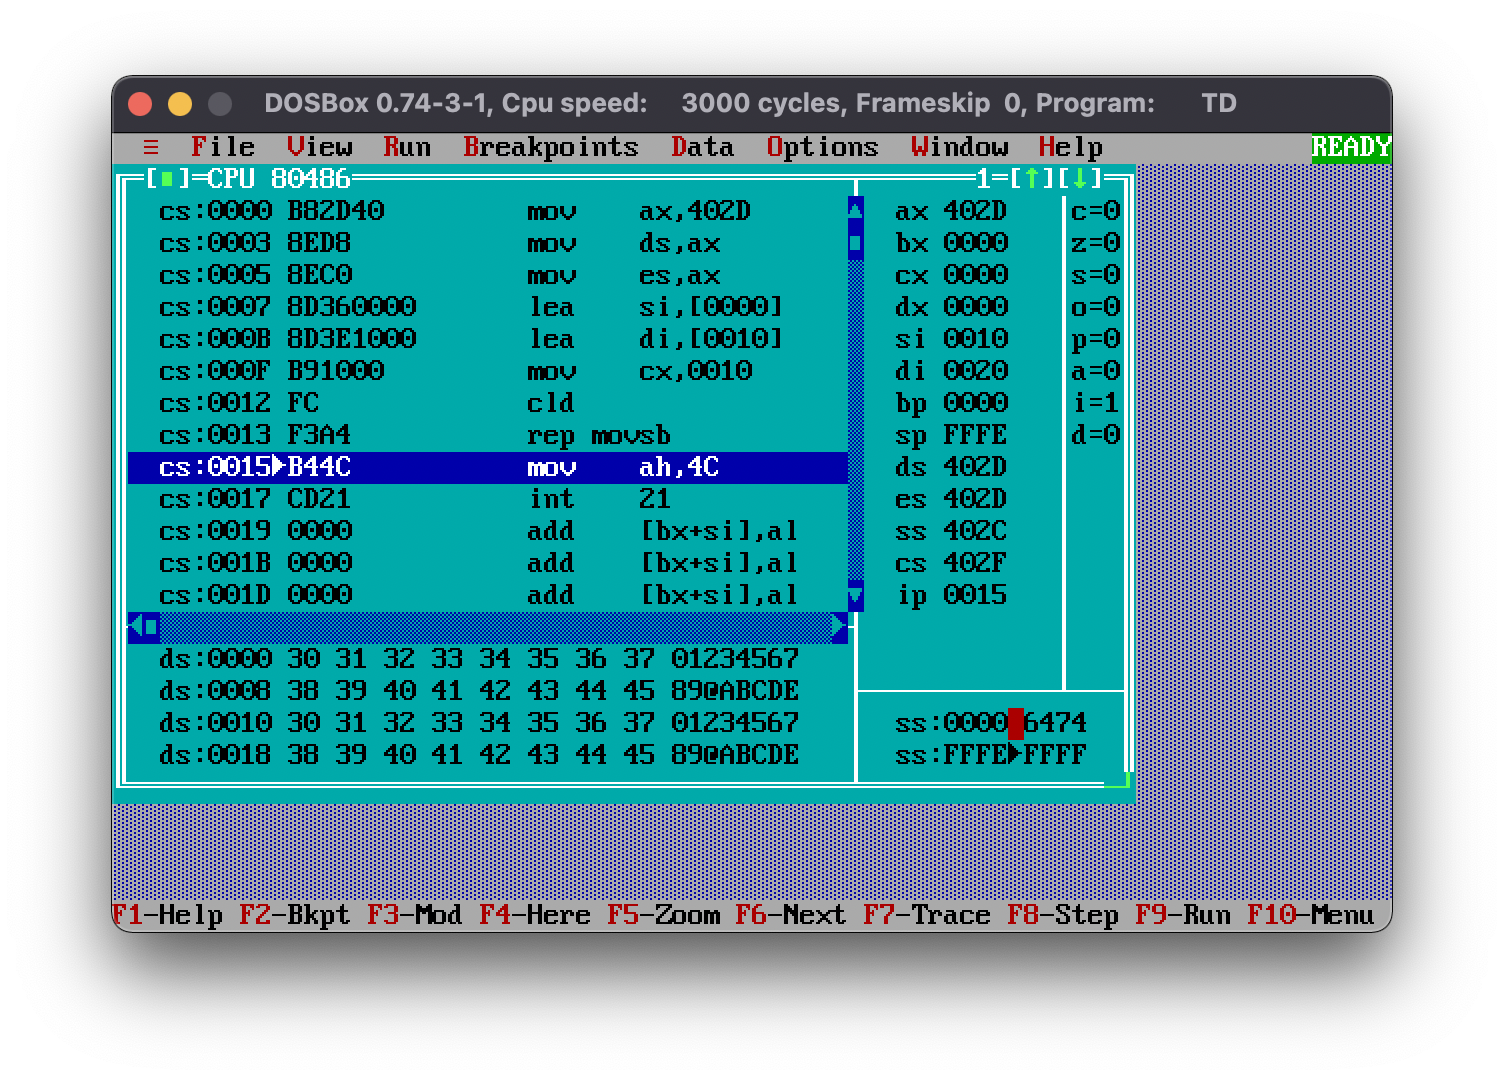
\includegraphics[width=0.7\textwidth]{fig/rlt55.png}
    \caption{实验结果}
    \label{fig:rlt55}
\end{figure}

\begin{note}{数据传送指令和串传送指令两种传送方式各自特点}{}
    数据传送指令需要定义两个指针,分别更新;串传送指令只需定义好源和目标的位置、长度,即可自动进行。
\end{note}

\subsection{实验六}
实验流程如图 \ref{fig:exp36}:
\begin{figure}[hbpt]
    \centering
    \begin{tikzpicture}[node distance = 2cm]
    \definecolor{myblued}{RGB}{0,114,189}
    \definecolor{myred}{RGB}{217,83,25}
    \definecolor{myyellow}{RGB}{237,137,32}
    \definecolor{mypurple}{RGB}{126,47,142}
    \definecolor{myblues}{RGB}{77,190,238}
    \definecolor{mygreen}{RGB}{32,134,48}
      \pgfplotsset{
        label style = {font=\fontsize{9pt}{7.2}\selectfont},
        tick label style = {font=\fontsize{7pt}{7.2}\selectfont}
      }
    
    \small  % 字体大小
    \tikzstyle{format}=[rectangle,draw,thin,fill=white]  % 定义语句块的颜色,形状和边
    % rectangle:矩形,可加圆角(rounded corners,逗号跟在形状后面即可)
    % trapezium:平行四边形
    % diamond:菱形
    \tikzstyle{test}=[diamond,aspect=2,draw,thin]  % 定义条件块的形状,颜色
    \tikzstyle{point}=[coordinate,on grid,]  % 像素点,用于连接转移线

    % 定义note
    \node[format](init){初始化数据段,将数据传入\texttt{DS}};
    \node[format,below of=init,node distance=10mm](1){定义数据指针\texttt{BX},设置循环次数};
    \node[format,below of=1,node distance=10mm](2){假设第一个数据是最大值,放入\texttt{AL}};
    \node[format,below of=2,node distance=10mm](3){\texttt{BX+1}};
    \node[format,below of=3,node distance=10mm](4){使用\texttt{CPM}指令比较数据,表现在标志位};
    \node[test,below of=4,node distance=20mm](5){\texttt{AL<[BX]?(有符号数比较)}};
    \node[format,below of=5,node distance=20mm](6){更新\texttt{AL}为\texttt{[BX]}};
    \node[test,below of=6,node distance=20mm](7){是否完成预设循环次数?};
    \node[format,below of=7,node distance=20mm](8){保存结果};
    \node[format,below of=8,node distance=10mm](end){结束,返回\texttt{DOS}};
    % 开始画线
    \draw[->](init)--(1);
    \draw[->](1)--(2);
    \draw[->](2)--(3);
    \draw[->](3)--(4);
    \draw[->](4)--(5);
    \draw[->](5)--node[left]{Yes}(6);
    \draw[->](6)--(7);
    \draw[->](7)--node[left]{Yes}(8);
    \draw[->](8)--(end);
    \draw[->](5.west) -+ (-4,-6) -+ node[left]{No}(-4,-10) -- (7.west);
    \draw[->](7.east) -+ (+4,-10) -+ node[right]{No}(+4,-3) -- (3.east);
\end{tikzpicture}

    \caption{执行流程}
    \label{fig:exp36}
\end{figure}

实验要求代码、正确结果(图\ref{fig:rlt6})如下:
\begin{lstlisting}[language={[x86masm]Assembler},title=exp36.asm]
    DATA   SEGMENT
    NUM    DB 22,46,32,72,84,16,156  ;定义数据段
    MAXN   DB ?  ;定义结果存放处
    DATA   ENDS

    MAIN SEGMENT 
    ASSUME CS:MAIN,DS:DATA
    START: MOV  AX,DATA
           MOV  DS,AX     ;DATA数据段传入DS
           LEA  BX,NUM    ;获取NUM偏移地址,传入指针BX
           MOV  CX,07     ;循环次数为7
           MOV  AL ,[BX]  ;初始假设第一个数据是最大值
    AGAIN: INC  BX        ;BX指针后移1位
           CMP  AL,[BX]   ;比较数据大小并更新标志位
           JNLE NEXT      ;如果AL>[BX],跳转至NEXT
           MOV  AL,[BX]   ;如果AL<[BX],更新AL
    NEXT:  LOOP AGAIN     ;循环CX次
           MOV  MAXN,AL   ;将结果存入MAXN
           MOV  AH,4CH
           INT  21H
    MAIN ENDS
    END START
\end{lstlisting}

\begin{figure}[htbp]
    \centering
    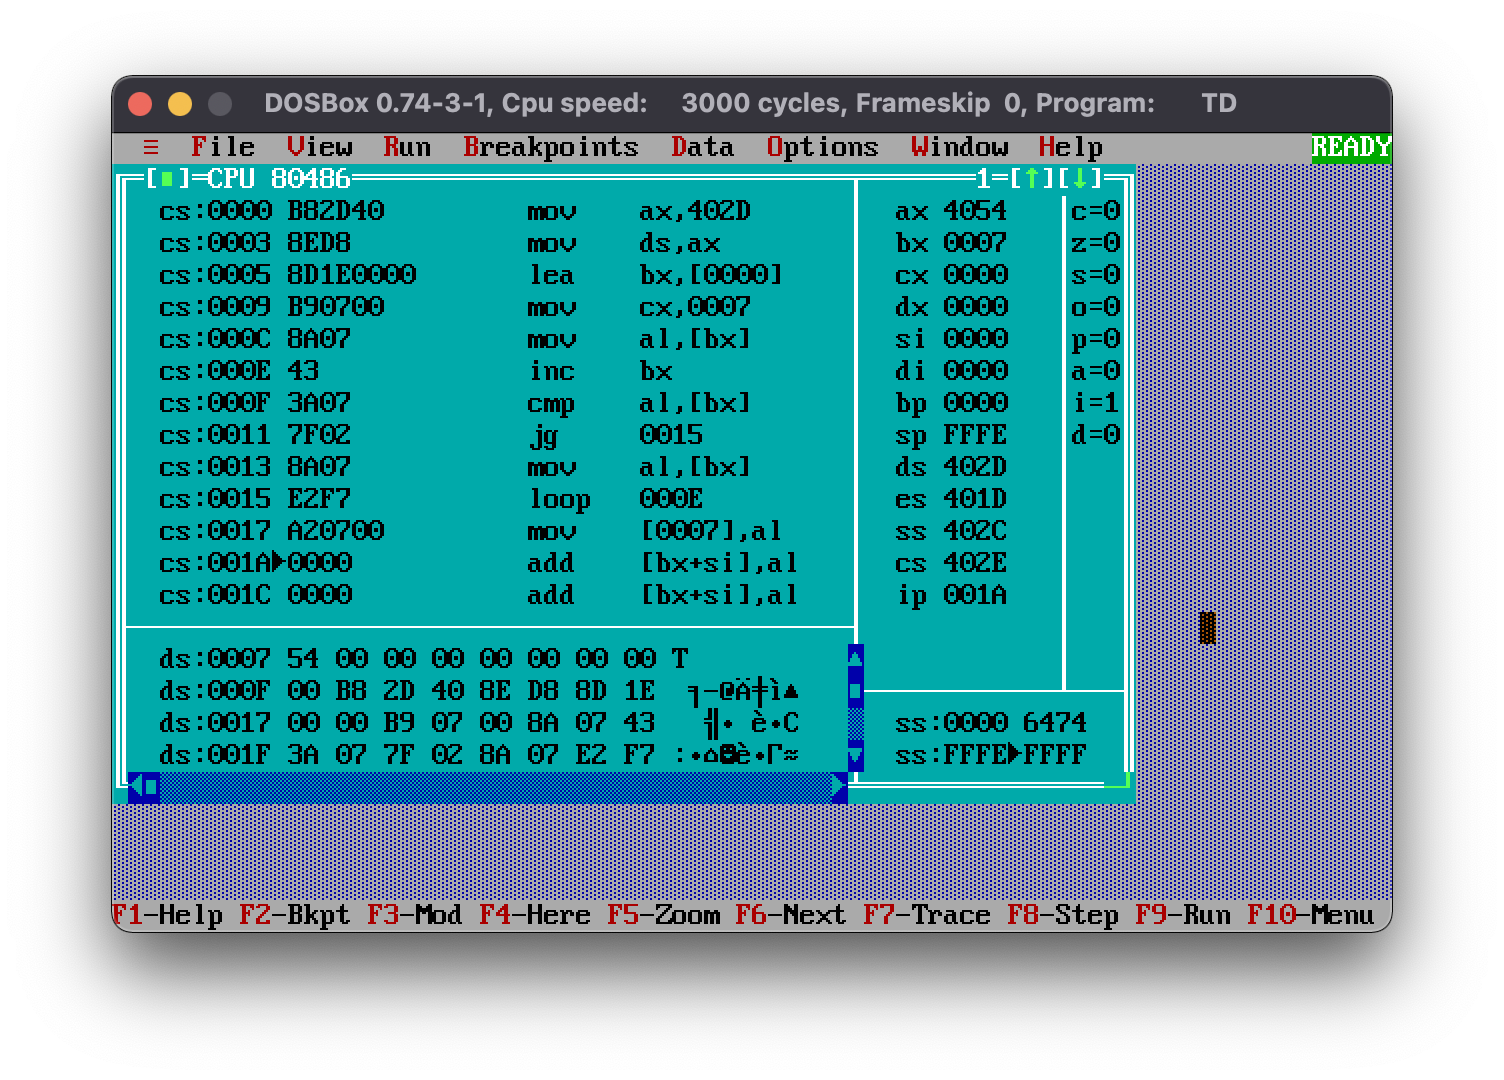
\includegraphics[width=0.7\textwidth]{fig/rlt6.png}
    \caption{实验结果}
    \label{fig:rlt6}
\end{figure}

\begin{note}{题目变化}{}
    只需要将比较大小改为有符号数的\texttt{JNLE}即可
\end{note}

\subsection{实验七}
实验流程如图 \ref{fig:exp37}:
\begin{figure}[hbpt]
    \centering
    \begin{tikzpicture}[node distance = 2cm]
    \definecolor{myblued}{RGB}{0,114,189}
    \definecolor{myred}{RGB}{217,83,25}
    \definecolor{myyellow}{RGB}{237,137,32}
    \definecolor{mypurple}{RGB}{126,47,142}
    \definecolor{myblues}{RGB}{77,190,238}
    \definecolor{mygreen}{RGB}{32,134,48}
      \pgfplotsset{
        label style = {font=\fontsize{9pt}{7.2}\selectfont},
        tick label style = {font=\fontsize{7pt}{7.2}\selectfont}
      }
    
    \small  % 字体大小
    \tikzstyle{format}=[rectangle,draw,thin,fill=white]  % 定义语句块的颜色,形状和边
    % rectangle:矩形,可加圆角(rounded corners,逗号跟在形状后面即可)
    % trapezium:平行四边形
    % diamond:菱形
    \tikzstyle{test}=[diamond,aspect=2,draw,thin]  % 定义条件块的形状,颜色
    \tikzstyle{point}=[coordinate,on grid,]  % 像素点,用于连接转移线

    % 定义note
    \node[format](init){初始化数据段,将数据传入\texttt{DS}};
    \node[format,below of=init,node distance=10mm](0){设置结果数组位置\texttt{[DI]}、被乘数数组的位置、循环次数,\textcolor{red}{结果存放指针\texttt{[DI]}直接指向末尾后一个字节,把\$放好}};
    \node[format,below of=0,node distance=10mm](1){倒退一字节,从最后一字节开始放结果};
    \node[format,below of=1,node distance=10mm](2){把此时指针所指的数字搬到\texttt{AL}};
    \node[format,below of=2,node distance=10mm](3){被乘数指针\texttt{+1}};
    \node[format,below of=3,node distance=10mm](4){进行相乘操作};
    \node[format,below of=4,node distance=10mm](5){非压缩\texttt{BCD}码的调整乘法};
    \node[format,below of=5,node distance=10mm](6){将[DI]中算出来的上一位的进位加上};
    \node[format,below of=6,node distance=10mm](7){非压缩\texttt{BCD}码的调整加法};
    \node[format,below of=7,node distance=10mm](8){调整好的正确的低位给了\texttt{[DI]},\textcolor{red}{并通过\texttt{+30}调整成\texttt{ASCII}码}};
    \node[format,below of=8,node distance=10mm](9){结果指针\textcolor{red}{\texttt{-1}}};
    \node[format,below of=9,node distance=10mm](10){把调整好的正确的进位给了\texttt{[DI]}};
    \node[test,below of=10,node distance=20mm](11){是否达到循环次数?};
    \node[format,below of=11,node distance=20mm](12){单独把最高位调整成\texttt{ASCII}码};
    \node[format,below of=12,node distance=10mm](13){设置打印开始位置,并打印};
    \node[format,below of=13,node distance=10mm](end){结束,返回\texttt{DOS}};
    % 开始画线
    \draw[->](init)--(0);
    \draw[->](0)--(1);
    \draw[->](1)--(2);
    \draw[->](2)--(3);
    \draw[->](3)--(4);
    \draw[->](4)--(5);
    \draw[->](5)--(6);
    \draw[->](6)--(7);
    \draw[->](7)--(8);
    \draw[->](8)--(9);
    \draw[->](9)--(10);
    \draw[->](10)--(11);
    \draw[->](11)--node[left]{Yes}(12);
    \draw[->](12)--(13);
    \draw[->](13)--(end);
    \draw[->](11.west) -+ (-6,-13) -+ node[left]{No}(-6,-3) -- (2.west);
\end{tikzpicture}

    \caption{执行流程}
    \label{fig:exp37}
\end{figure}

实验要求代码、正确结果(图\ref{fig:rlt7})如下:
\begin{lstlisting}[language={[x86masm]Assembler},title=exp37.asm]
    DATA   SEGMENT
DATA1  DB 08,04,03,03,05
DATA2  DB 09
SUM    DB 6 DUP(00)   ;把00复制6次,占用6个BYTE
DATA   ENDS 
    
CODE SEGMENT
ASSUME CS:CODE,DS:DATA
START:  MOV AX,DATA          
        MOV DS,AX             ;手动分配段地址
        MOV SI,OFFSET DATA2   ;DATA2的偏移地址给了SI
        MOV DL,[SI]           ;把SI内所指向的存储器的内容给了DL
        MOV SI,OFFSET DATA1   ;DATA1的偏移地址给了SI
        MOV DI,OFFSET SUM     ;SUM的偏移地址给了DI
        ADD DI,6              ;调整指针指到末尾(已经出了数据段,是放$的地方)
        MOV [DI],24H          ;$放在最后
        DEC DI                ;开始从开辟的SUN空间的最后一个开始计算
        MOV CX,05             ;循环次数为5
NEXT:   MOV AL,[SI]           ;一位位开始算,先从第一位开始
        INC SI                ;指针加一,指向下一位
        MUL DL                ;和09相乘
        AAM                   ;非压缩BCD码的乘法调整指令
        ADD AL,[DI]           ;[DI]中有上一个算出来的进位,
                              ;先把进位加上
        AAA                   ;调整成非压缩BCD码
        MOV [DI],AL           ;调整好之后,把正确的低位给了AL
        ADD [DI],30H          ;换算成ASCII码
        DEC DI                ;存放下一个数字的位置
        MOV [DI],AH           ;把上一个调整产生的进位放到DI中
        LOOP NEXT
        ADD [DI],30H          ;换算成ASCII码
        MOV DX,OFFSET SUM     ;设置字符串的首地址为打印首地址
        MOV AH,09H
        INT 21H               ;打印
        MOV AH,4CH
        INT 21H
CODE ENDS
END START    

\end{lstlisting}

\begin{figure}[htbp]
    \centering
    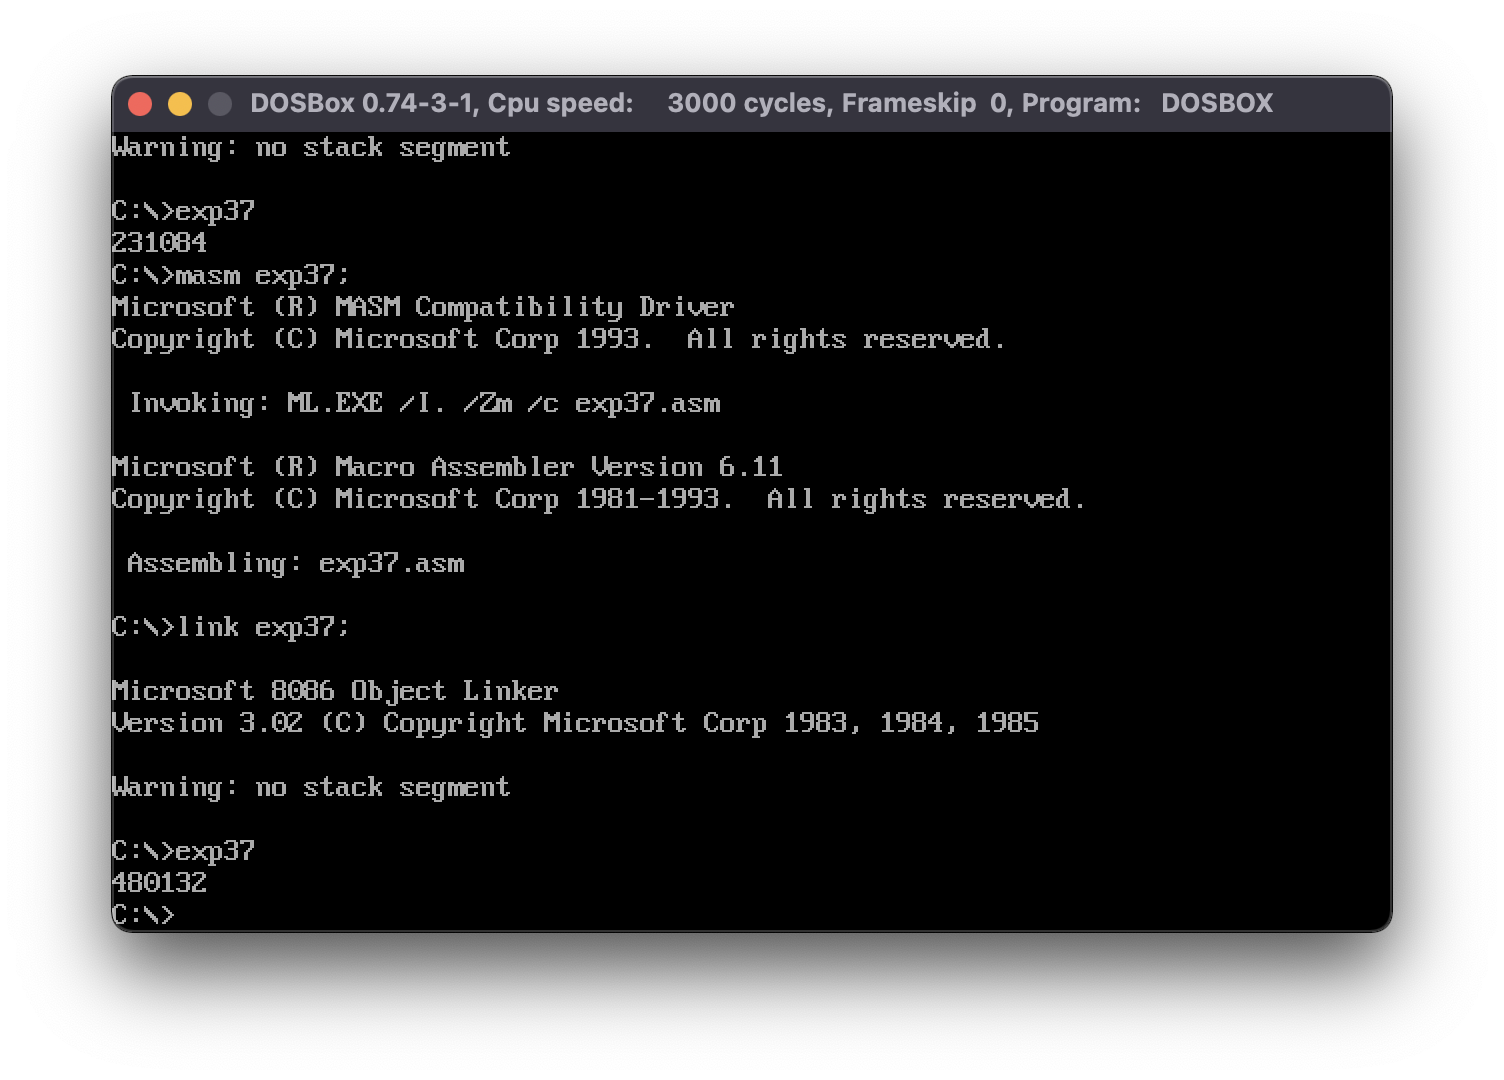
\includegraphics[width=0.7\textwidth]{fig/rlt7.png}
    \caption{实验结果}
    \label{fig:rlt7}
\end{figure}

\begin{note}{字符串顺序相反问题}{}
    由于高位放在高地址,但是打印是从地位开始,所以会造成结果相反的情况,一种解决方案是先开辟SUM空间,然后直接挪到最后,把'\$'放好,然后逆着求解,最后正着打印。
\end{note}

\section{思考题}
\begin{enumerate}
    \item 在例题中,\texttt{CMP BL,00}指令有何作用?\\
    通过比较\texttt{BL}中元素与\texttt{00}的大小来影响标志位,从而影响负数个数计数器的值。
    \item \texttt{CMP BL,00}指令是否可以用其它指令代替?\\
    可以。通过\texttt{SUB BL,00}来判断是是否为负数。
    \item 无符号数和有符号数比较大小时,用到的条件跳转指令有何不同?\\
    无符号数大于用\texttt{JNBE};有符号数大于用\texttt{JNLE}。
    \item 在例题程序(求负数个数)的数据段中,如果要用符号定义伪指令\texttt{EQU}定义一个常量\texttt{N}表示数据缓冲区\texttt{NUM}的字节数,请写出相应的伪指令。\\
    \begin{lstlisting}[language={[x86masm]Assembler},title=code]
    N EQU $-NUM
    \end{lstlisting}
    \item 在例题程序(求负数个数)中,指令\texttt{LEA SI,NUM}中,源操作数是什么寻址方式?该指令可用什么指令替换?\\
    立即数寻址;可以使用\texttt{LEA SI,OFFSET NUM}。
    \item 实验任务4中,非压缩\texttt{BCD}码乘法和加法分别用了什么调整指令?简要说明非压缩\texttt{BCD}码乘法和加法调整指令的调整方法。并写出执行该程序进行$(53348\times 9)$的乘法运算时,第一次执行乘法的BCD码调整指令后的调整结果和第一次执行加法的\texttt{BCD}码调整指令后的调整结果。\\
    \texttt{AAM}和\texttt{AAA},\texttt{AAM}:将\texttt{AL}除以\texttt{10},商放\texttt{AH},余数\texttt{AL};\texttt{AAA}:若\texttt{AL}低4位大于9或\texttt{AF=1},\texttt{AH+1},\texttt{AL+6},将\texttt{AF}和\texttt{CF}置1,再清除\texttt{AL}高四位;执行完成的结果都是\texttt{AX=0702}。
    \item 请说明在串操作时,方向标志DF的作用,并分别写出DF清零和置1的指令。\\
    \texttt{DF=0},指针增加,否则减小。

\end{enumerate}

\section{实验总结}
实验总结已随文附在“注意”、“思考”、“分析”中。

% 打印参考文献
\addcontentsline{toc}{section}{参考文献}
\printbibliography

\end{document}
